\section{Graphics Processing Units}
\label{sec:GPU}
Dedicated \glspl{gpu} are very common in desktop and laptops. \citep{STEAMHW}
GPUs are commonly used in the private and professional world, for computer gaming and accelerating graphic intensive programs such as Adobe Photoshop and 3D modelling tools. \citep{NVIDIAADOBE}
Their architecture can also be used for advantageously for certain types of computations, primarily computations which can be done in parallel. 
An example of this can be calculating different properties of the pixels on a screen. 
The screen can then be divided into different sections and the computations for each section is divided over the GPU.
This is possible because the calculations do not require results from the other calculations.
Unlike the cores in the CPU the cores in the GPU are not optimized for sequential serial processing, instead its cores are designed to handle multiple tasks at once. 
As such running sequential code on the CPU will be more efficient, where as more compute-intensive functions may be better suited for the GPU.\citep{NvidiaGPGPU}
The before mentioned example can be viewed as a matrix being divided into sections, so the same method of parallelised workflow can be applied when multiplying two matrices.

\begin{figure}[h!]
\centering
 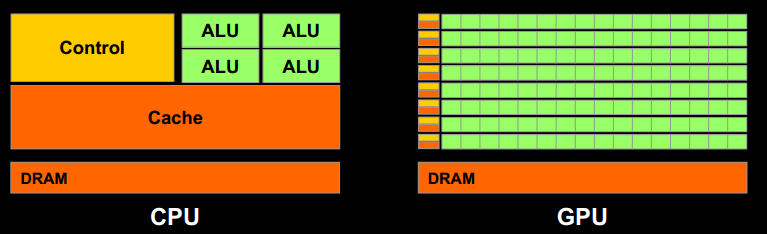
\includegraphics[width=1\textwidth]{figures/GPUCPUimage.png} % trim=4.85cm 15cm 0.85cm 1cm
\caption{A basic representation of the Transistor allocation on a GPU compared to a CPU}\label{image:GPUCPUimage}\citep{NvidiaCUDASeminar}
\vspace{-15pt}
\end{figure}

A simple representational comparison of a Central Processing Unit's - CPU - and a GPU's transistor usage is shown in \myref{image:GPUCPUimage}.
The GPU consists of more less powerful cores where as the CPU consists of fewer more powerful ones, the greater amount of cores allows for more computation power.
As of Q1 2015 an example of a modern high end desktop CPU is the Intel Haswell core i7 5960X which has 8 cores. \citep{puget}
A contemporary high end GPU is the NVIDIA GTX 980 which has 2048 CUDA cores. \citep{techpowerup,gtx980}
Due to their architectural differences the GPU allows for about 12 times more operations per second.

This makes the GPU particularly useful for computation, even some which are not graphical. % Antagende/konkluderende?!?



 for simpler problems, where as more complex problems can prove difficult. \todo{Expand on this(Interesting)} 